\scanpage{7}
\figure{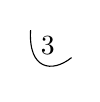
\begin{tikzpicture}[x=1cm,y=1cm]\node at (0,0) {\mspage{3}};\draw (-.22,.2) .. controls (-.25,-.3) and (.05,-.35) .. (.3,-.15);\end{tikzpicture}}
2) \uline{Foncteur ess. surjectif}
\margin{\fbox{\parbox{.6\linewidth}{\uline{Si} $S$ \uline{géom. unibranche en les points de} $S-U$ (\unsure{.}\par et si le normalisé de $S_{\mathrm{red}}$ est \unsure{fini} sur $S$.}}}
\margin{[plus gén., si, posant $S''=S'\times_S S'$, $U'=U\times_S S'$, $U''=U\times_S S''$, $U^{(\unsure{n})}$ \deleted{\unsure{rencontre}} rencontre ttes comp$^{\unsure{\mathrm{tes}}}$ connexes de $S^{(\unsure{n})}$]}
\figure{\begin{tikzpicture}[x=1cm,y=1cm]\draw[->] (0,0)--(-.45,0);\draw[->] (4.8,-2.1)..controls(4.4,-1.3)and(6,.1)..(5,0);\end{tikzpicture}}
\deleted{a) \unsure{Supposons}}
Partant de $A_U,M,\varphi$, on veut construire $A$.
\inserted{On peut supposer $S$ affine, $S=\operatorname{Spec}\Lambda$.}
\deleted{Par descente, il suffit de \unsure{traiter ce cas}.}

a) Réduction au cas $S$ réduit.

Soit $S_0=S_{\mathrm{red}}$, $A_0$ schéma abélien sur $S_0$ qui y résout le pb. Par Serre-Tate, on trouve \deleted{\unsure{des}}\inserted{\deleted{\unsure{un}}} schémas abéliens sur les $T_n$, donc un schéma \inserted{formel} abélien \inserted{$A'$} sur $S'=\unsure{\operatorname{Spec}}\hat\Lambda$. Son image inverse sur $S'_0$ est un vrai schéma abélien, \deleted{\unsure{sur $S$}} \unsure{savoir} l'image inverse de $A_0$ sur $S'_0$. Donc (réf \dots !!!) $A'$ provient d'un vrai schéma abélien $A'$ sur $S'$ [l'immersion $S'_0\mathbin{-}S'$ étant nilpotente]. Or $U\amalg S'\to S$ est fid. plat, et on trouve une donnée de descente sur $A_U\amalg A'$. Elle \unsure{devient} effective après dépt de base $S_0\hookrightarrow S$, donc elle l'était déjà avant, d'après le critère de Raynaud. On gagne !
\margin{\unsure{?}}
\margin{\diagram{\begin{tikzcd}[ampersand replacement=\&,column sep=small,row sep=small]
S_0\arrow[d] \& S'_0\arrow[l]\arrow[d]\\
S \& S'\arrow[l]
\end{tikzcd}}}

\deleted{b) Réduction au cas $S$ local, \deleted{\unsure{et de}} $T=$ point fermé.
Pour faire cette réduction, on est amené à prouver ceci: si $t$ est un pt \unsure{maximal|général} de $T$, $V$ un ouvert contenant $t$ et $U$, \deleted{et} $A_V$ un schéma abélien sur $V$ \deleted{qui \unsure{induit}} $M$ par sa restriction à $S'=\operatorname{Spec}\underline O_{S,t}$ \deleted{\unsure{vérifie}} est OK, alors $A_V$ est \deleted{\unsure{encore}} OK dans un voisinage, i.e. l'isom donné $T_p(A_{S'})\simeq M_{S'}$ se prolonge en un isom en un}
\margin{?}
\mspage{6}
